\documentclass[10pt]{scrreprt}
\usepackage[utf8]{inputenc}
\usepackage{amsmath}
\usepackage{amsfonts}
\usepackage{amssymb}
\usepackage{graphicx}
\author{Kim Rostgaard Christensen}
\title{Requirements as tests}
\subtitle{Automatic generation of test from structured requirements}

\begin{document}
\maketitle

\begin{abstract}
The world of software is has over the years been tainted with stories about failed projects. Almost everyone has his or her on story about a given software system, that did not solve the task, which it was designed to. This indicates; either a mismatch between requirements and solution, or simply erroneous requirement specifications.
\end{abstract}

\chapter{Introduction}
The natural evolution of software engineering points towards increasing the level of abstraction, moving closer to the usage models that they try capture. Another benefit of using models is that they communicate much better than, for instance, source code. Whereas source code is usually filled with non-essential implementation-specific details, models aim only to capture the essence of what it represents. Models, lacking these details, are challenging to execute. An doing so requires a great deal of extra work, filling out the details with either code snibblets or equivalent constraints -- such as OCL.\footnote{Object Constraint Language - part of UML}\\\\
One problem with this approach is a that much technical knowledge is required to formulate the models, OCL constraints and/or snibblets required for the system to function. For most technical staff it feels like meta-programming that keeps them from doing real programming.
\\\\
Ideally, the person requesting the software being modeled (the customer), should do a lot of the modeling by him/herself. This, however, has historically proven itself infeasible as customers rarely know much about modeling or programming, and if they did, would probably not be requesting software but rather making it on their own.
\\\\
This thesis will try to look for a middle ground, where we put the customer in the middle and try to provide a tool and methodology to extract models and verification information from them indirectly. The hope is to be able to infer or manually add semantics to the system descriptions the users provide, so that we will be able to generate acceptance tests from them.
\section{Terminology}
\subsection{Three kinds of models}
This document will use three descriptions for models, which cover;
\subsubsection{Informal models}
Informal models are used to describe models whose primary purpose is serve as a communication or documentation tool, not have strict semantics and cannot be used for code generation or model-checking.
\subsubsection{Formal models}
Formal models, which can be used for verification -- such as Z or VDM or plain math. Anything that has strict semantics and can be used to unambiguously generate code.
\subsubsection{Meta-models}
Meta-models that model other models, such as UML.


\chapter{Case project}
This project uses the open source project ``OpenReception'' as case study. The project aims to provide a drop-in replacement for an existing system, and therefore has relatively fixed requirements that are extracted from the workings of the existing system. The system is open source and any implementation details are therefore public domain. This section gives a short introduction to the system and


\begin{figure}
  \centering
 
  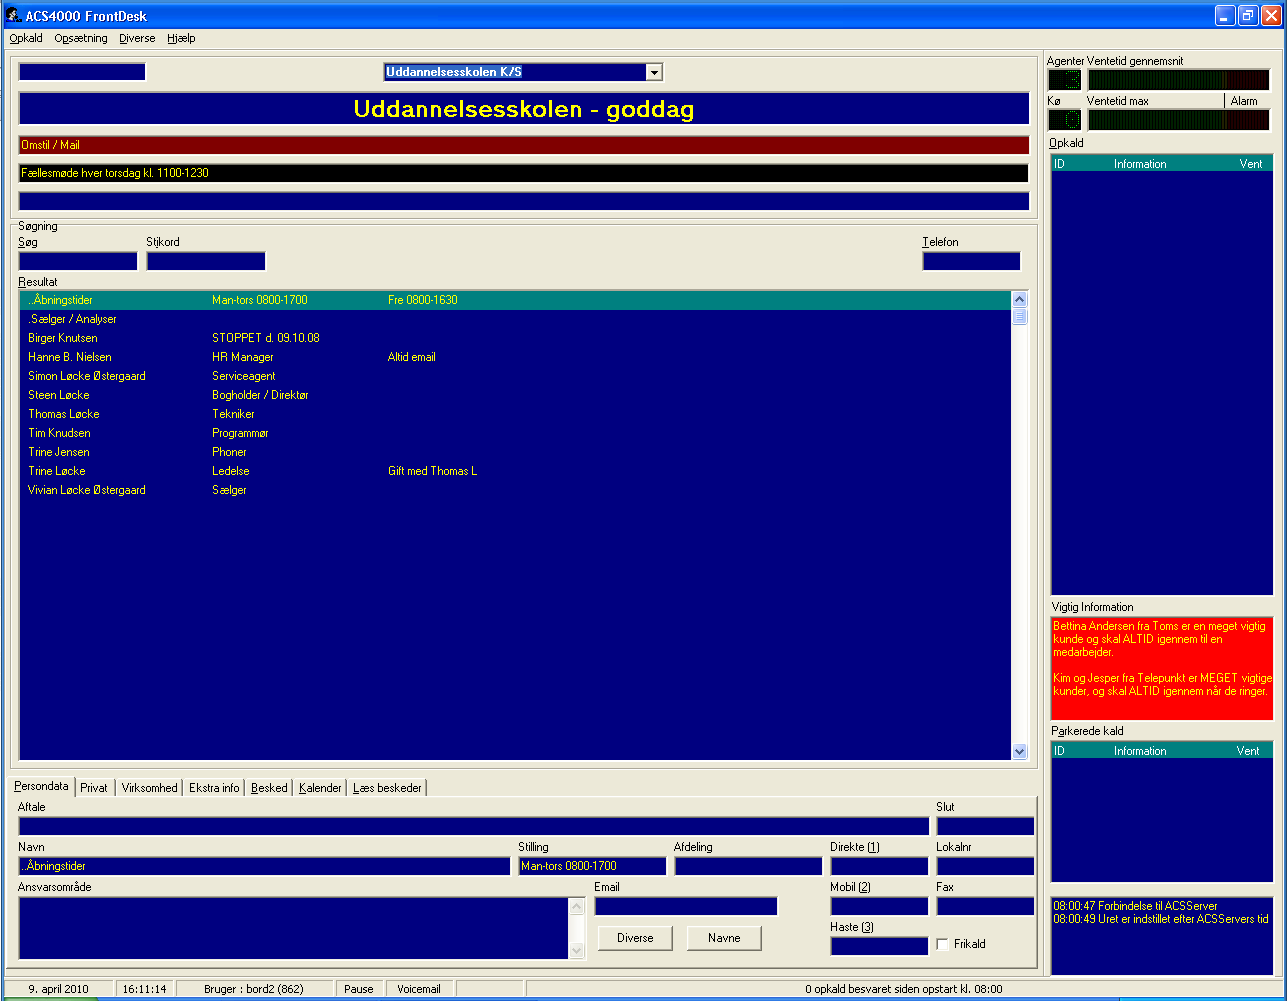
\includegraphics[scale=0.2]{img/frontdesk-client-ui.png}
  \caption{Receptionist client user interface of existing system}
  \label{fig:frontdesk-client-ui}
\end{figure}

\begin{figure}
  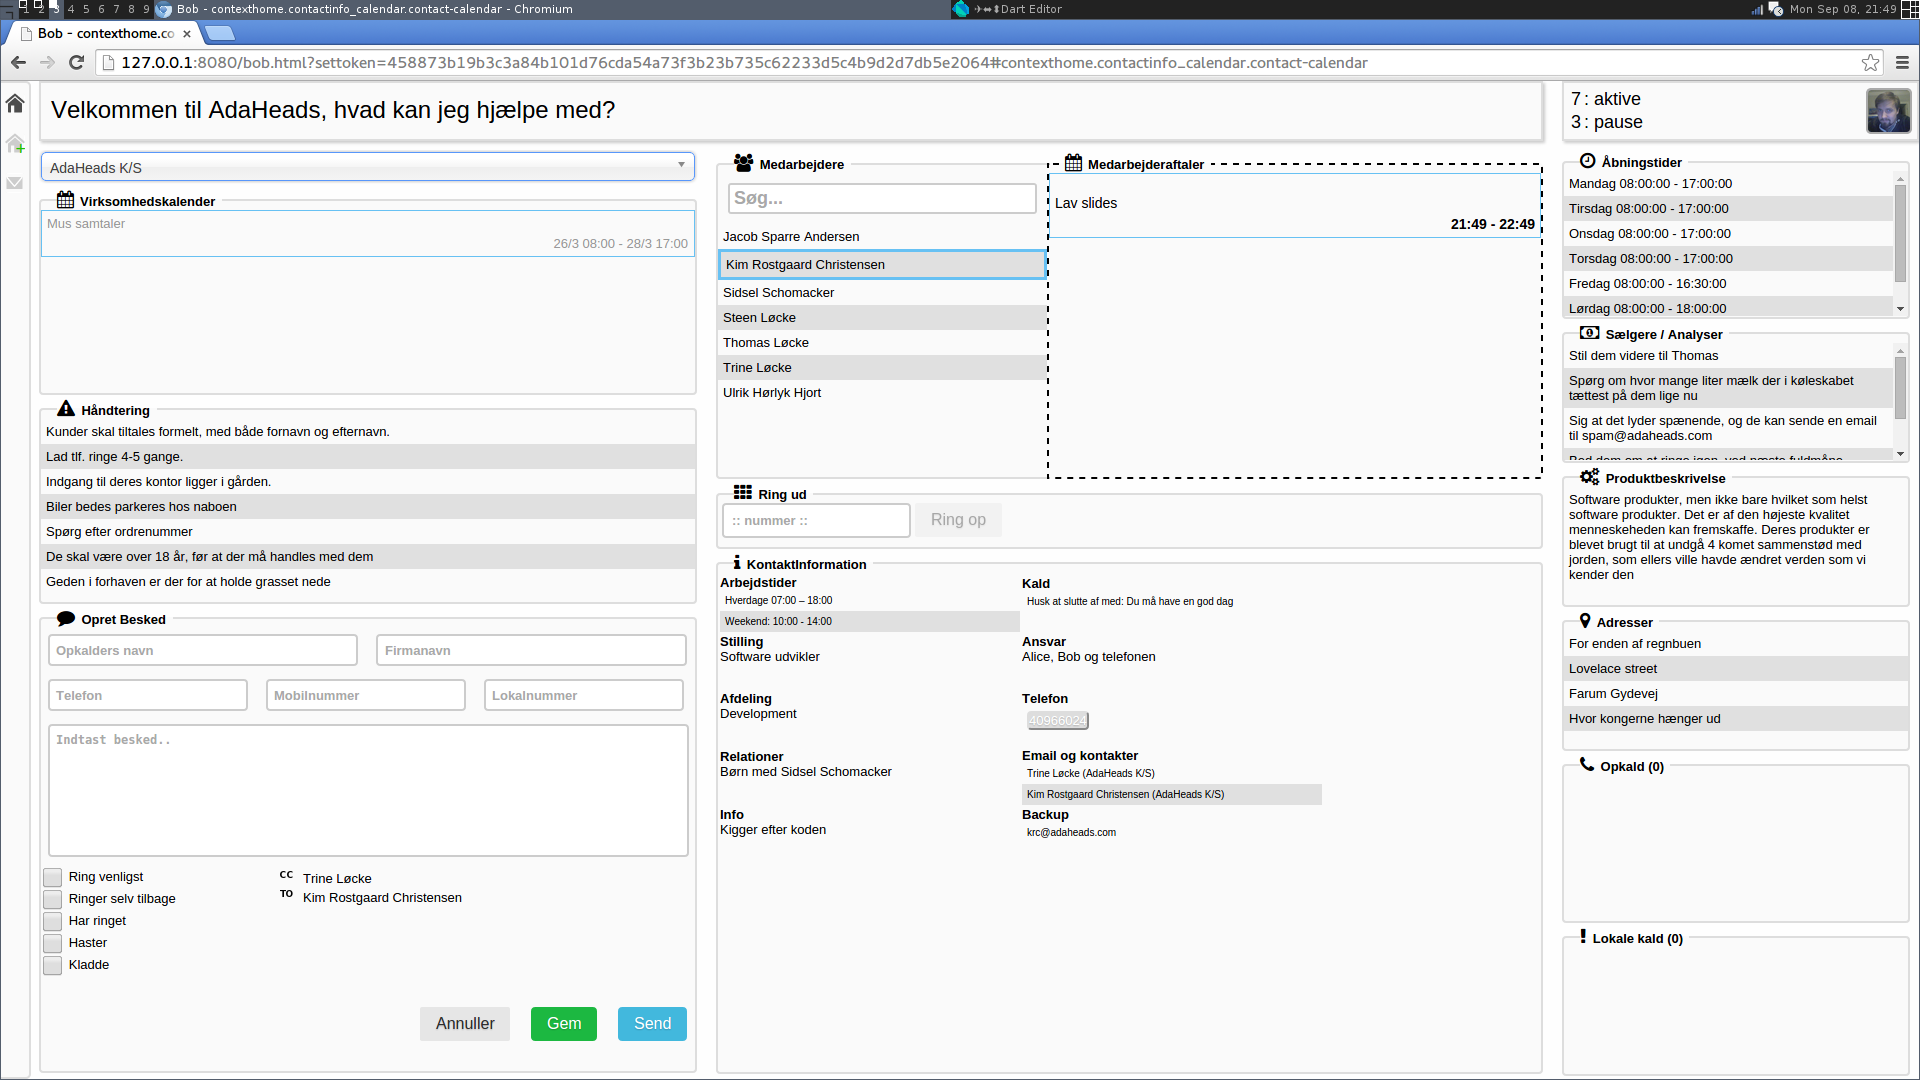
\includegraphics[scale=0.2]{img/openreception-client-ui.png}
  \caption{Receptionist client user interface of OpenReception system}
  \label{fig:openreception-client-ui}
\end{figure}

\section{Brainstorming}
The problem in attaining broad coverage of use cases, and therefore completeness in requirements i primarily that, from the customer perspective, that they feel very overly-verbose and usually too formal in nature. For software engineers, the opposite is usually the case. They feel that the use case descriptions are not structured nor elaborate enough for use in, for instance, code stub generation.

More structure, however, could be helped along the way with proper tooling. Hiding some of the complexity of the constrains of a data model behind a simple user interface supplying dragable components and providing immediate visual feedback in the form of textual use case representation (or a diagram) could "cheat" the customer into adding the needed structure to the use case model.

\begin{figure}[h]
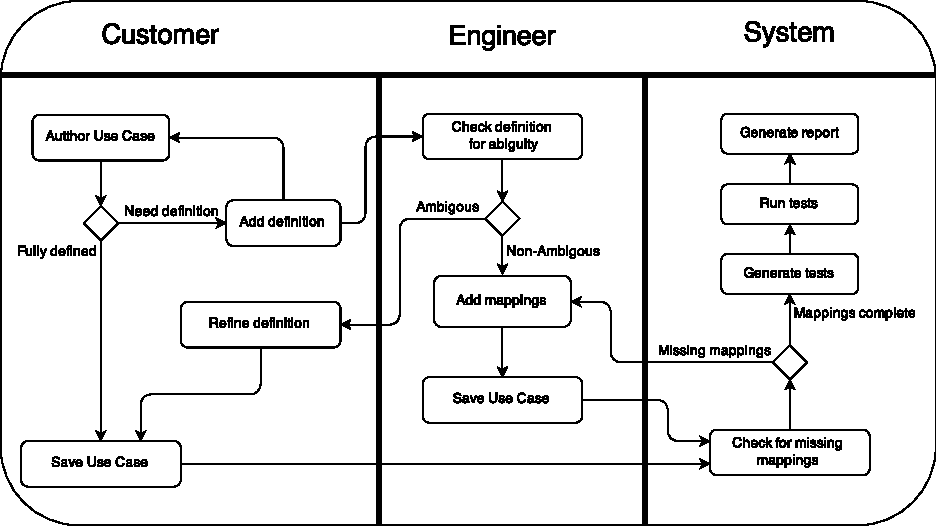
\includegraphics[scale=0.9]{img/use_case_creation_activity_diagram}
\centering
\caption{Use case creation with different actors}
\label{fig:use_case_creation_activity_diagram}
\end{figure}

What is in the customers interest is having acceptance tests match the use cases as closely as possible. Preferably, the should be able to be automated as well. Figure \ref{fig:use_case_creation_activity_diagram} shows an activity diagram involving three actors, the customer, the engineer and the system\footnote{Use case system}. In this diagram, the customer authors use cases while adding missing definitions not already in the tool. A definition is textual description of a concept which may be -- for instance -- an actor, role or action. This description is then given a unique name, that may correspond to a concept already found in the domain model. The domain model, if defined beforehand, could also be thought to be a part of the built-in declarations.

\begin{figure}[h]
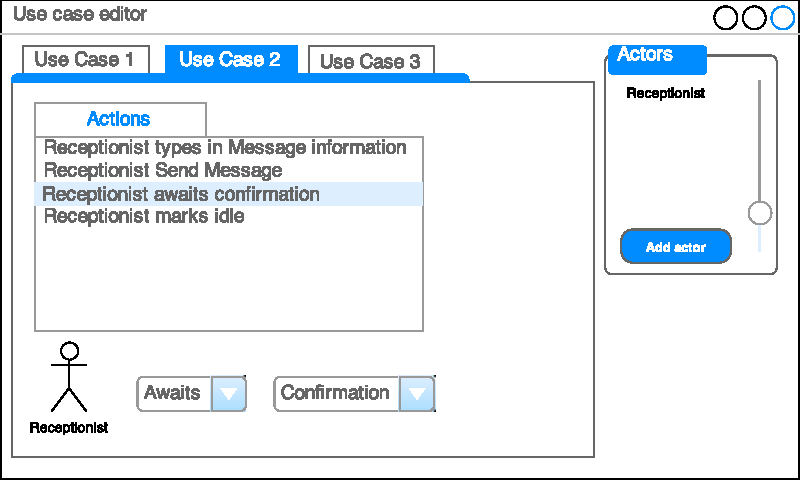
\includegraphics[scale=0.9]{img/test_case_ui}
\centering
\caption{Use case editor UI mockup}
\label{fig:use_case_editor_mockup}
\end{figure}

Whenever there is a new use case, a change to an existing use case, or simply a definition, the system should try to generate tests from the new information. If this step fails it is likely due to insufficient concept mappings. From here, a software engineer must manually map individual definitions to system macro-functionality or, possibly the use case could be linked to an existing manually written test, if the generation step is not possible for some reason. A mockup of a user interface is shown in figure \ref{fig:use_case_editor_mockup}.

% Something about generating partially-automated tests, where the system sets up everything for the customer and then notifies them about the next steps they have to take to move the test forward.

\section{Glossary}
\subsection{Customer}
The person in the role of purchasing the software. Assumed to have little or no knowledge about formalism, modeling or programming.

\section{Extracting semantic}
Example; in the use case it is stated that a call is hung up and a callee awaits this event. The lifeline of the call is however not tracked and to be able to properly assert the true state of this, the code macro needs to into account this lifeline and reflect on which assertions hold for every stakeholder that has knowledge of the call. % TODO: Elaborate the example and explain that a phone call is a good example because it has an A and B-leg and potentially a system that tracks its state.

\subsection{Letting the customer inject semantics}

There are two basic approaches to letting the customer inject semantics into the requirements. The first is to do a full up-front declaration of every term used within the problem domain and supply this as a toolbox for the customer %todo example.
The other approach is to do it on the go by outlining concepts as stubs whenever they appear. This approach is similar to what is used in wiki software. %todo eaxmple

\section{Verification problem}
A big issue in software

\section{End-user experience}
%The challenge in documenting requirements is, and has always been, to formulate them on a non-ambiguous form. The quantification of ambiguity tends to be difficult as well, due to the fact that requirements are usually formulated in natural languages following some rules, such as pre-defined glossary and constraints. Constraints vocabulary typically consists of should, could, may, must.

%As requirements are basically constraints to your system, a subset of them may be expressed as expressions following a formality that is machine-interpretable. Vienna Development Method (VDM) and Z notation are two approaches that tries to formally describe systems on a very high level, so that model-checking can be performed on it prior to programming.

An example UI is Starting from scratch, the user would be expected to initially define at least one actor and add a sequence of actions that the actor perform.

%Other method
Wiki-collaboration to "lazily" define the problem domain and verification conditions along the way.

\section{Test setup}
%scaffolding and harness

\section{Formulating requirements}

\section{Requirements as communication platform}

Avoid technical jargon (\cite{christel1992issues})

\section{Related work}
\subsection{FIT Framework}





\section{Use case writing level}
Should not be used to describe UI actions% http://alistair.cockburn.us/Use+cases%2c+ten+years+later (Use case limits).

Use cases expresses expected system behavior. Keep use cases free of UI-action.

There are several levels on which use cases can be written as per\cite{cockburn??}. In our case, it would make the most sense to use the "system" level, as business level is something that is nearly useless because it is largely out of scope. The business logic is also, more elaborately (and implicitly) formulated within a system-level use case. In the other end, a component use case is also very impractical, as our target audience would be people that does not know anything about the specifics of the system being built.


\section{Expressing requirements}

\section{Targeted requirements}
We've chosen to focus on the requirements that involves core features from the Receptionist actor point of view. These are, on a high level;
\begin{description}
  \item[Manage calls:] Being able to technically handle calls by performing receive, park, transfer and hangup action.
  \item[Process calls:] Being able to process calls in the context of a dialed reception. This involves having access to data about the reception and its contacts. Being able to dial them, or send them a message.
  \item[Manage message:] Being able to send out messages to contacts, view and resend existing messages.
\end{description}

This gives the following -- more detailed -- requirements
\begin{description}
  \item[RQ1: Transfer to contact:] A receptionist must be able to transfer a call to a chosen contact associated with the currently active reception. An example use case, from the receptionist actor point of view is outlined below.
  \begin{itemize}
    \item Preconditions.
    \begin{itemize}
      \item Receptionist has previously received a call $A$
      \item Receptionist has parked the previously received call $A$
    \end{itemize}
    \item Actions.
    \begin{itemize}
      \item Receptionist dials the number of the selected contact (call $B$)
      \item Receptionist hears dial tone
      \item The contact's phone is ringing.
      \item The contact accepts the calls (picks up)
      \item Receptionist has a dialogue with contact
      \item Receptionist transfers call $B$ to call $A$
      \item The system breaks the receptionist's connection to both call $A$ and $B$    
      \item Receptionist marks his/her state as idle.
    \end{itemize}
  \end{itemize}

  \item[RQ2: Send message to contact:] A receptionist must be able to send a message -- via a distribution list -- to a contact, typically containing information received verbally via a call. An example use case, from the receptionist actor point of view is outlined below.
  \begin{itemize}
    \item Preconditions.
    \begin{itemize}
      \item Receptionist may have previously received a call $A$, which may still be active.
    \end{itemize}
    \item Actions.
    \begin{itemize}
      \item Receptionist finds contact $C$ who will serve as recipient
      \item Receptionist selects $C$
      \item Receptionist types in message
      \item Receptionist sends the message via the system
      \item Receptionist marks his/her state as idle.
    \end{itemize}
  \end{itemize}
\end{description}

%TODO High leve description (customer level)

\chapter{Validating implementation}
%Something about the V-model.

\section{Formalized approaches}
%2.1. Use case description
%A semiformal use case description is simply a natural
%language text structured using a text template which divides
%the text into logical parts. Even though there is no broadly
%accepted standard use case template, the existing templates
%are quite similar.
\section{Testing}
%Fixtures
%Design by contract
%Harness

\section{Regression testing}

\chapter{Requirement formalization}
Actors, Roles

Aspects. Behavior. State space.

\section{Use case as base}
\includegraphics[scale=0.4]{img/req_meta.png}

\section{Processes}

\chapter{Test generation}
Using -- exclusively -- the use case from \textbf{RQ2} as base, we try to derive what is needed in order to generate a basic test.
To achieve the minimum implementation, we cut away the optional precondition that may be covered by other use cases. After this, we see an implicitly \emph{ordered list of actions} that we need to succeed in order for the test to be a success. There is an actor that performs an action at each step. The system, in its entirety, may also be referred to as an actor as it is also capable of performing actions.

So, summing up, we have;
\begin{itemize}
  \item This use case consists of an ordered list of actions, where actions consist of
  \begin{itemize}
	\item One or more actors
	\item One verb describing the action
	\item One target for the action (object for verb)
  \end{itemize}
\end{itemize}
If we 

\section{Requirement/test mapping}
The communication model needs to be known.

\chapter{Process evaluation}

\chapter{Conclusion}


% PROJECT DESCRIPTION BELOW.


\section*{Background}
Within software projects, documented requirements often become outdated and irrelevant over time as requirements are implemented and verified manually. For long-lived projects that continuously add features and components, maintenance of requirements becomes increasingly cumbersome, and increases the risk of requirement documentation decay further. Dynamic documents -- for instance, an inter-linked web document written in wiki markup -- may make requirement maintenance more accessible. This applies to both humans, but especially also for computers that may extract valuable information about system requirements for use in system verification tests.\\\\
Additionally, if the requirements are formalized in a sufficiently structured way, and annotated with references to the implementation, the cost of requirements maintenance may be made worthwhile by enabling us to automatically generate system tests from them.
\subsection*{Project}
The key idea is that sufficient structure in requirement formalization may enable tests to be generated directly from requirements fully automatically. To facilitate this, it means that requirements should be written with a strong focus on testability. This, as a side effect, may increase the motivation for quantifying, constraining and refining requirements. As an example: \emph{Who} will perform this action, and how are the outcomes expected to be presented/received?\\\\
The project will use the requirements from an existing system as a case study and formalize the structure of these, so that test generation from them is possible. During this process, we will investigate how to structure requirements so that we can generate tests directly from them and map implementation to requirements. Ideally, we want to identify general patterns and constraints in the structure/formalism introduced to our requirements in the case study, to be able to apply them to other projects. But in general, we will investigate to which extent this idea can be applied.
%In the software engineering field, a paradigm shift from waterfall-oriented development methods, towards more agile and iterative methods. However, the iterative approach still has a requirements phase, that may play an only minor role in the implementation phase, and focus shifts to \emph{how to make it work}, rather than \emph{what it should do}. Test-driven development handles this pragmatically by enforcing that tests are written before implementations. This provides a strong interface-driven black-box oriented methodology. It also provides a feedback channel for requirement changes.\\\\
%Taking test-driven development a step further, one may perceive the software system in its entirety as a large interface, and it's requirements as the tests. Use cases are textual descriptions of the functional requirements of the system, which are typically written in a semi-formal language, using only terms clearly defined within a domain model or glossary.\\
%Applying transformations to use cases derived from requirements, turning them into automated acceptance tests, could provide a more requirement-oriented development method, keeping the requirements in the loop during the entire development process.

%\section{Project}
%The approach motioned above is influenced by model driven development, formal methods
%\begin{itemize}
%  \item Identify generalizable traits of automated acceptance test generation from a case study focusing on the constraints/complexity reduction tradeoff.
%  \item Establish a process for identifying requirements, research and possibly create methods for formalizing them
%  \item Build a proof-of-concept tool for generating tests from use cases
  %\item Evaluate the value of the approach.
%\end{itemize}
%A growing numer of software systems are being moved to the cloud, which makes it a lot easier to make "rolling releases", rather than monolithic releases. %TODO More

%During the development of the OpenReception project, the team have applied a number of ah-hoc measures to 

\bibliographystyle{plain}
\bibliography{references}

\nocite{*}

\end{document}